% Options for packages loaded elsewhere
% Options for packages loaded elsewhere
\PassOptionsToPackage{unicode}{hyperref}
\PassOptionsToPackage{hyphens}{url}
\PassOptionsToPackage{dvipsnames,svgnames,x11names}{xcolor}
%
\documentclass[
  twoside,
  symmetric]{tufte-book}
\usepackage{xcolor}
\usepackage{amsmath,amssymb}
\setcounter{secnumdepth}{-\maxdimen} % remove section numbering
\usepackage{iftex}
\ifPDFTeX
  \usepackage[T1]{fontenc}
  \usepackage[utf8]{inputenc}
  \usepackage{textcomp} % provide euro and other symbols
\else % if luatex or xetex
  \usepackage{unicode-math} % this also loads fontspec
  \defaultfontfeatures{Scale=MatchLowercase}
  \defaultfontfeatures[\rmfamily]{Ligatures=TeX,Scale=1}
\fi
\usepackage{lmodern}
\ifPDFTeX\else
  % xetex/luatex font selection
\fi
% Use upquote if available, for straight quotes in verbatim environments
\IfFileExists{upquote.sty}{\usepackage{upquote}}{}
\IfFileExists{microtype.sty}{% use microtype if available
  \usepackage[]{microtype}
  \UseMicrotypeSet[protrusion]{basicmath} % disable protrusion for tt fonts
}{}
\makeatletter
\@ifundefined{KOMAClassName}{% if non-KOMA class
  \IfFileExists{parskip.sty}{%
    \usepackage{parskip}
  }{% else
    \setlength{\parindent}{0pt}
    \setlength{\parskip}{6pt plus 2pt minus 1pt}}
}{% if KOMA class
  \KOMAoptions{parskip=half}}
\makeatother
% Make \paragraph and \subparagraph free-standing
\makeatletter
\ifx\paragraph\undefined\else
  \let\oldparagraph\paragraph
  \renewcommand{\paragraph}{
    \@ifstar
      \xxxParagraphStar
      \xxxParagraphNoStar
  }
  \newcommand{\xxxParagraphStar}[1]{\oldparagraph*{#1}\mbox{}}
  \newcommand{\xxxParagraphNoStar}[1]{\oldparagraph{#1}\mbox{}}
\fi
\ifx\subparagraph\undefined\else
  \let\oldsubparagraph\subparagraph
  \renewcommand{\subparagraph}{
    \@ifstar
      \xxxSubParagraphStar
      \xxxSubParagraphNoStar
  }
  \newcommand{\xxxSubParagraphStar}[1]{\oldsubparagraph*{#1}\mbox{}}
  \newcommand{\xxxSubParagraphNoStar}[1]{\oldsubparagraph{#1}\mbox{}}
\fi
\makeatother


\usepackage{longtable,booktabs,array}
\usepackage{calc} % for calculating minipage widths
% Correct order of tables after \paragraph or \subparagraph
\usepackage{etoolbox}
\makeatletter
\patchcmd\longtable{\par}{\if@noskipsec\mbox{}\fi\par}{}{}
\makeatother
% Allow footnotes in longtable head/foot
\IfFileExists{footnotehyper.sty}{\usepackage{footnotehyper}}{\usepackage{footnote}}
\makesavenoteenv{longtable}
\usepackage{graphicx}
\makeatletter
\newsavebox\pandoc@box
\newcommand*\pandocbounded[1]{% scales image to fit in text height/width
  \sbox\pandoc@box{#1}%
  \Gscale@div\@tempa{\textheight}{\dimexpr\ht\pandoc@box+\dp\pandoc@box\relax}%
  \Gscale@div\@tempb{\linewidth}{\wd\pandoc@box}%
  \ifdim\@tempb\p@<\@tempa\p@\let\@tempa\@tempb\fi% select the smaller of both
  \ifdim\@tempa\p@<\p@\scalebox{\@tempa}{\usebox\pandoc@box}%
  \else\usebox{\pandoc@box}%
  \fi%
}
% Set default figure placement to htbp
\def\fps@figure{htbp}
\makeatother


% definitions for citeproc citations
\NewDocumentCommand\citeproctext{}{}
\NewDocumentCommand\citeproc{mm}{%
  \begingroup\def\citeproctext{#2}\cite{#1}\endgroup}
\makeatletter
 % allow citations to break across lines
 \let\@cite@ofmt\@firstofone
 % avoid brackets around text for \cite:
 \def\@biblabel#1{}
 \def\@cite#1#2{{#1\if@tempswa , #2\fi}}
\makeatother
\newlength{\cslhangindent}
\setlength{\cslhangindent}{1.5em}
\newlength{\csllabelwidth}
\setlength{\csllabelwidth}{3em}
\newenvironment{CSLReferences}[2] % #1 hanging-indent, #2 entry-spacing
 {\begin{list}{}{%
  \setlength{\itemindent}{0pt}
  \setlength{\leftmargin}{0pt}
  \setlength{\parsep}{0pt}
  % turn on hanging indent if param 1 is 1
  \ifodd #1
   \setlength{\leftmargin}{\cslhangindent}
   \setlength{\itemindent}{-1\cslhangindent}
  \fi
  % set entry spacing
  \setlength{\itemsep}{#2\baselineskip}}}
 {\end{list}}
\usepackage{calc}
\newcommand{\CSLBlock}[1]{\hfill\break\parbox[t]{\linewidth}{\strut\ignorespaces#1\strut}}
\newcommand{\CSLLeftMargin}[1]{\parbox[t]{\csllabelwidth}{\strut#1\strut}}
\newcommand{\CSLRightInline}[1]{\parbox[t]{\linewidth - \csllabelwidth}{\strut#1\strut}}
\newcommand{\CSLIndent}[1]{\hspace{\cslhangindent}#1}



\setlength{\emergencystretch}{3em} % prevent overfull lines

\providecommand{\tightlist}{%
  \setlength{\itemsep}{0pt}\setlength{\parskip}{0pt}}



 


\hypersetup{colorlinks}
\usepackage{lipsum}
\usepackage{booktabs}
\usepackage{graphicx}
\setkeys{Gin}{width=\linewidth,totalheight=\textheight,keepaspectratio}
\graphicspath{{style-guide/graphics/}}
\usepackage{fancyvrb}
\fvset{fontsize=\normalsize}
\newcommand{\hangp}[1]{\makebox[0pt][r]{(}#1\makebox[0pt][l]{)}}
\newcommand{\hangstar}{\makebox[0pt][l]{*}}
\usepackage{xspace}
\newcommand{\vdqi}{\textit{VDQI}\xspace}
\newcommand{\ei}{\textit{EI}\xspace}
\newcommand{\ve}{\textit{VE}\xspace}
\newcommand{\be}{\textit{BE}\xspace}
\newcommand{\VDQI}{\textit{The Visual Display of Quantitative Information}\xspace}
\newcommand{\EI}{\textit{Envisioning Information}\xspace}
\newcommand{\VE}{\textit{Visual Explanations}\xspace}
\newcommand{\BE}{\textit{Beautiful Evidence}\xspace}
\newcommand{\TL}{Tufte-\LaTeX\xspace}
\newcommand{\monthyear}{%
  \ifcase\month\or January\or February\or March\or April\or May\or June\or
  July\or August\or September\or October\or November\or
  December\fi\space\number\year
}
\newcommand{\openepigraph}[2]{%
  \begin{fullwidth}
  \sffamily\large
  \begin{doublespace}
  \noindent\allcaps{#1}\\
  \noindent\allcaps{#2}
  \end{doublespace}
  \end{fullwidth}
}
\newcommand{\blankpage}{\newpage\hbox{}\thispagestyle{empty}\newpage}
\usepackage{units}
\newcommand{\measure}[3]{#1/#2$\times$\unit[#3]{pc}}
\newcommand{\hlred}[1]{\textcolor{Maroon}{#1}}
\newcommand{\hangleft}[1]{\makebox[0pt][r]{#1}}
\newcommand{\hairsp}{\hspace{1pt}}
\newcommand{\hquad}{\hskip0.5em\relax}
\newcommand{\TODO}{\textcolor{red}{\bf TODO!}\xspace}
\newcommand{\na}{\quad--}
\providecommand{\XeLaTeX}{X\lower.5ex\hbox{\kern-0.15em\reflectbox{E}}\kern-0.1em\LaTeX}
\newcommand{\tXeLaTeX}{\XeLaTeX\index{XeLaTeX@\protect\XeLaTeX}}
\newcommand{\tuftebs}{\symbol{'134}}
\newcommand{\doccmdnoindex}[2][]{\texttt{\tuftebs#2}}
\newcommand{\doccmddef}[2][]{%
  \hlred{\texttt{\tuftebs#2}}\label{cmd:#2}%
  \ifthenelse{\isempty{#1}}%
    {\index{#2 command@\protect\hangleft{\texttt{\tuftebs}}\texttt{#2}}}%
    {\index{#2 command@\protect\hangleft{\texttt{\tuftebs}}\texttt{#2} (\texttt{#1} package)}%
     \index{#1 package@\texttt{#1} package}\index{packages!#1@\texttt{#1}}}%
}
\newcommand{\doccmd}[2][]{%
  \texttt{\tuftebs#2}%
  \ifthenelse{\isempty{#1}}%
    {\index{#2 command@\protect\hangleft{\texttt{\tuftebs}}\texttt{#2}}}%
    {\index{#2 command@\protect\hangleft{\texttt{\tuftebs}}\texttt{#2} (\texttt{#1} package)}%
     \index{#1 package@\texttt{#1} package}\index{packages!#1@\texttt{#1}}}%
}
\newcommand{\docopt}[1]{\ensuremath{\langle}\textrm{\textit{#1}}\ensuremath{\rangle}}
\newcommand{\docarg}[1]{\textrm{\textit{#1}}}
\newenvironment{docspec}{\begin{quotation}\ttfamily\parskip0pt\parindent0pt\ignorespaces}{\end{quotation}}
\newcommand{\docenv}[1]{\texttt{#1}\index{#1 environment@\texttt{#1} environment}\index{environments!#1@\texttt{#1}}}
\newcommand{\docenvdef}[1]{\hlred{\texttt{#1}}\label{env:#1}\index{#1 environment@\texttt{#1} environment}\index{environments!#1@\texttt{#1}}}
\newcommand{\docpkg}[1]{\texttt{#1}\index{#1 package@\texttt{#1} package}\index{packages!#1@\texttt{#1}}}
\newcommand{\doccls}[1]{\texttt{#1}}
\newcommand{\docclsopt}[1]{\texttt{#1}\index{#1 class option@\texttt{#1} class option}\index{class options!#1@\texttt{#1}}}
\newcommand{\docclsoptdef}[1]{\hlred{\texttt{#1}}\label{clsopt:#1}\index{#1 class option@\texttt{#1} class option}\index{class options!#1@\texttt{#1}}}
\newcommand{\docmsg}[2]{\bigskip\begin{fullwidth}\noindent\ttfamily#1\end{fullwidth}\medskip\par\noindent#2}
\newcommand{\docfilehook}[2]{\texttt{#1}\index{file hooks!#2}\index{#1@\texttt{#1}}}
\newcommand{\doccounter}[1]{\texttt{#1}\index{#1 counter@\texttt{#1} counter}}
\usepackage{makeidx}
\makeindex
\makeatletter
\@ifpackageloaded{caption}{}{\usepackage{caption}}
\AtBeginDocument{%
\ifdefined\contentsname
  \renewcommand*\contentsname{Table of contents}
\else
  \newcommand\contentsname{Table of contents}
\fi
\ifdefined\listfigurename
  \renewcommand*\listfigurename{List of Figures}
\else
  \newcommand\listfigurename{List of Figures}
\fi
\ifdefined\listtablename
  \renewcommand*\listtablename{List of Tables}
\else
  \newcommand\listtablename{List of Tables}
\fi
\ifdefined\figurename
  \renewcommand*\figurename{Figure}
\else
  \newcommand\figurename{Figure}
\fi
\ifdefined\tablename
  \renewcommand*\tablename{Table}
\else
  \newcommand\tablename{Table}
\fi
}
\@ifpackageloaded{float}{}{\usepackage{float}}
\floatstyle{ruled}
\@ifundefined{c@chapter}{\newfloat{codelisting}{h}{lop}}{\newfloat{codelisting}{h}{lop}[chapter]}
\floatname{codelisting}{Listing}
\newcommand*\listoflistings{\listof{codelisting}{List of Listings}}
\makeatother
\makeatletter
\makeatother
\makeatletter
\@ifpackageloaded{caption}{}{\usepackage{caption}}
\@ifpackageloaded{subcaption}{}{\usepackage{subcaption}}
\makeatother
\makeatletter
\@ifpackageloaded{sidenotes}{}{\usepackage{sidenotes}}
\@ifpackageloaded{marginnote}{}{\usepackage{marginnote}}
\makeatother
\usepackage{bookmark}
\IfFileExists{xurl.sty}{\usepackage{xurl}}{} % add URL line breaks if available
\urlstyle{same}
\hypersetup{
  pdftitle={A Tufte-Style Book},
  pdfauthor={The Tufte-LaTeX Developers},
  colorlinks=true,
  linkcolor={blue},
  filecolor={Maroon},
  citecolor={Blue},
  urlcolor={Blue},
  pdfcreator={LaTeX via pandoc}}


\title{A Tufte-Style Book}
\usepackage{etoolbox}
\makeatletter
\providecommand{\subtitle}[1]{% add subtitle to \maketitle
  \apptocmd{\@title}{\par {\large #1 \par}}{}{}
}
\makeatother
\subtitle{Thanks to Edward R. Tufte for his inspiration}
\author{The Tufte-LaTeX Developers}
\date{2025-05-25}
\begin{document}
\frontmatter
\maketitle

\renewcommand*\contentsname{Table of contents}
{
\hypersetup{linkcolor=}
\setcounter{tocdepth}{2}
\tableofcontents
}
\listoffigures
\listoftables

\mainmatter
\chapter*{Introduction}\label{introduction}
\addcontentsline{toc}{chapter}{Introduction}

This sample book discusses the design of Edward Tufte's books(Tufte
2001, 1990, 1997, 2006) and the use of the \texttt{tufte-book} and
\texttt{tufte-handout} document classes.

\chapter{The Design of Tufte's Books}\label{ch:tufte-design}

\newthought{The pages} of a book are usually divided into three major
sections: the front matter (also called preliminary matter or prelim),
the main matter (the core text of the book), and the back matter (or end
matter).

\newthought{The front matter} of a book refers to all of the material
that comes before the main text. The following table shows a list of
material that appears in the front matter of \VDQI, \EI, \VE, and
\BE along with its page number. Page numbers that appear in parentheses
refer to folios that do not have a printed page number (but they are
still counted in the page number sequence).

\bigskip
\begin{minipage}{\textwidth}
\begin{center}
\begin{tabular}{lcccc}
\toprule
 & \multicolumn{4}{c}{Books} \\
\cmidrule(l){2-5} 
Page content & \vdqi & \ei & \ve & \be \\
\midrule
Blank half title page & \hangp{1} & \hangp{1} & \hangp{1} & \hangp{1} \\
Frontispiece\footnotemark{} & \hangp{2} & \hangp{2} & \hangp{2} & \hangp{2} \\
Full title page & \hangp{3} & \hangp{3} & \hangp{3} & \hangp{3} \\
Copyright page & \hangp{4} & \hangp{4} & \hangp{4} & \hangp{4} \\
Contents & \hangp{5} & \hangp{5} & \hangp{5} & \hangp{5} \\
Dedication & \hangp{6} & \hangp{7} & \hangp{7} & 7 \\
Epigraph & -- & -- & \hangp{8} & -- \\
Introduction & \hangp{7} & \hangp{9} & \hangp{9} & 9 \\
\bottomrule
\end{tabular}
\end{center}
\end{minipage}
\footnotetext{The contents of this page vary from book to book. In \vdqi this page is blank; in \ei and \ve this page holds a frontispiece; and in \be this page contains three epigraphs.}

\bigskip

The design of the front matter in Tufte's books varies slightly from the
traditional design of front matter. First, the pages in front matter are
traditionally numbered with lowercase roman numerals (e.g., i, ii, iii,
iv, \ldots). Second, the front matter page numbering sequence is usually
separate from the main matter page numbering. That is, the page numbers
restart at 1 when the main matter begins. In contrast, Tufte has
enumerated his pages with arabic numerals that share the same page
counting sequence as the main matter.

There are also some variations in design across Tufte's four books. The
page opposite the full title page (labeled ``frontispiece'' in the above
table) has different content in each of the books. In \VDQI, this page
is blank; in \EI and \VE, this page holds a frontispiece; and in \BE,
this page contains three epigraphs.

The dedication appears on page 6 in \vdqi (opposite the introduction),
and is placed on its own spread in the other books. In \ve, an epigraph
shares the spread with the opening page of the introduction.

None of the page numbers (folios) of the front matter are expressed
except in \be, where the folios start to appear on the dedication page.

\newthought{The full title page} of each of the books varies slightly in
design. In all the books, the author's name appears at the top of the
page, the title is set just above the center line, and the publisher is
printed along the bottom margin. Some of the differences are outlined in
the following table.

\bigskip
\begin{center}
\footnotesize
\begin{tabular}{lllll}
\toprule
Feature & \vdqi & \ei & \ve & \be \\
\midrule
Author & & & & \\
\quad Typeface & serif   & serif   & serif   & sans serif \\
\quad Style    & italics & italics & italics & upright, caps \\
\quad Size     & 24 pt   & 20 pt   & 20 pt   & 20 pt \\
\addlinespace
Title & & & & \\
\quad Typeface & serif   & serif   & serif   & sans serif \\
\quad Style    & upright & italics & upright & upright, caps \\
\quad Size     & 36 pt   & 48 pt   & 48 pt   & 36 pt \\
\addlinespace
Subtitle & & & & \\
\quad Typeface & \na     & \na     & serif   & \na \\
\quad Style    & \na     & \na     & upright & \na \\
\quad Size     & \na     & \na     & 20 pt   & \na \\
\addlinespace
Edition & & & & \\
\quad Typeface & sans serif    & \na  & \na  & \na \\
\quad Style    & upright, caps & \na  & \na  & \na \\
\quad Size     & 14 pt         & \na  & \na  & \na \\
\addlinespace
Publisher & & & & \\
\quad Typeface & serif   & serif   & serif   & sans serif \\
\quad Style    & italics & italics & italics & upright, caps \\
\quad Size     & 14 pt   & 14 pt   & 14 pt   & 14 pt \\
\bottomrule
\end{tabular}
\end{center}

\begin{figure*}


\includegraphics[width=0.45\linewidth,height=\textheight,keepaspectratio]{style-guide/graphics/vdqi-title.pdf}

\includegraphics[width=0.45\linewidth,height=\textheight,keepaspectratio]{style-guide/graphics/ei-title.pdf}

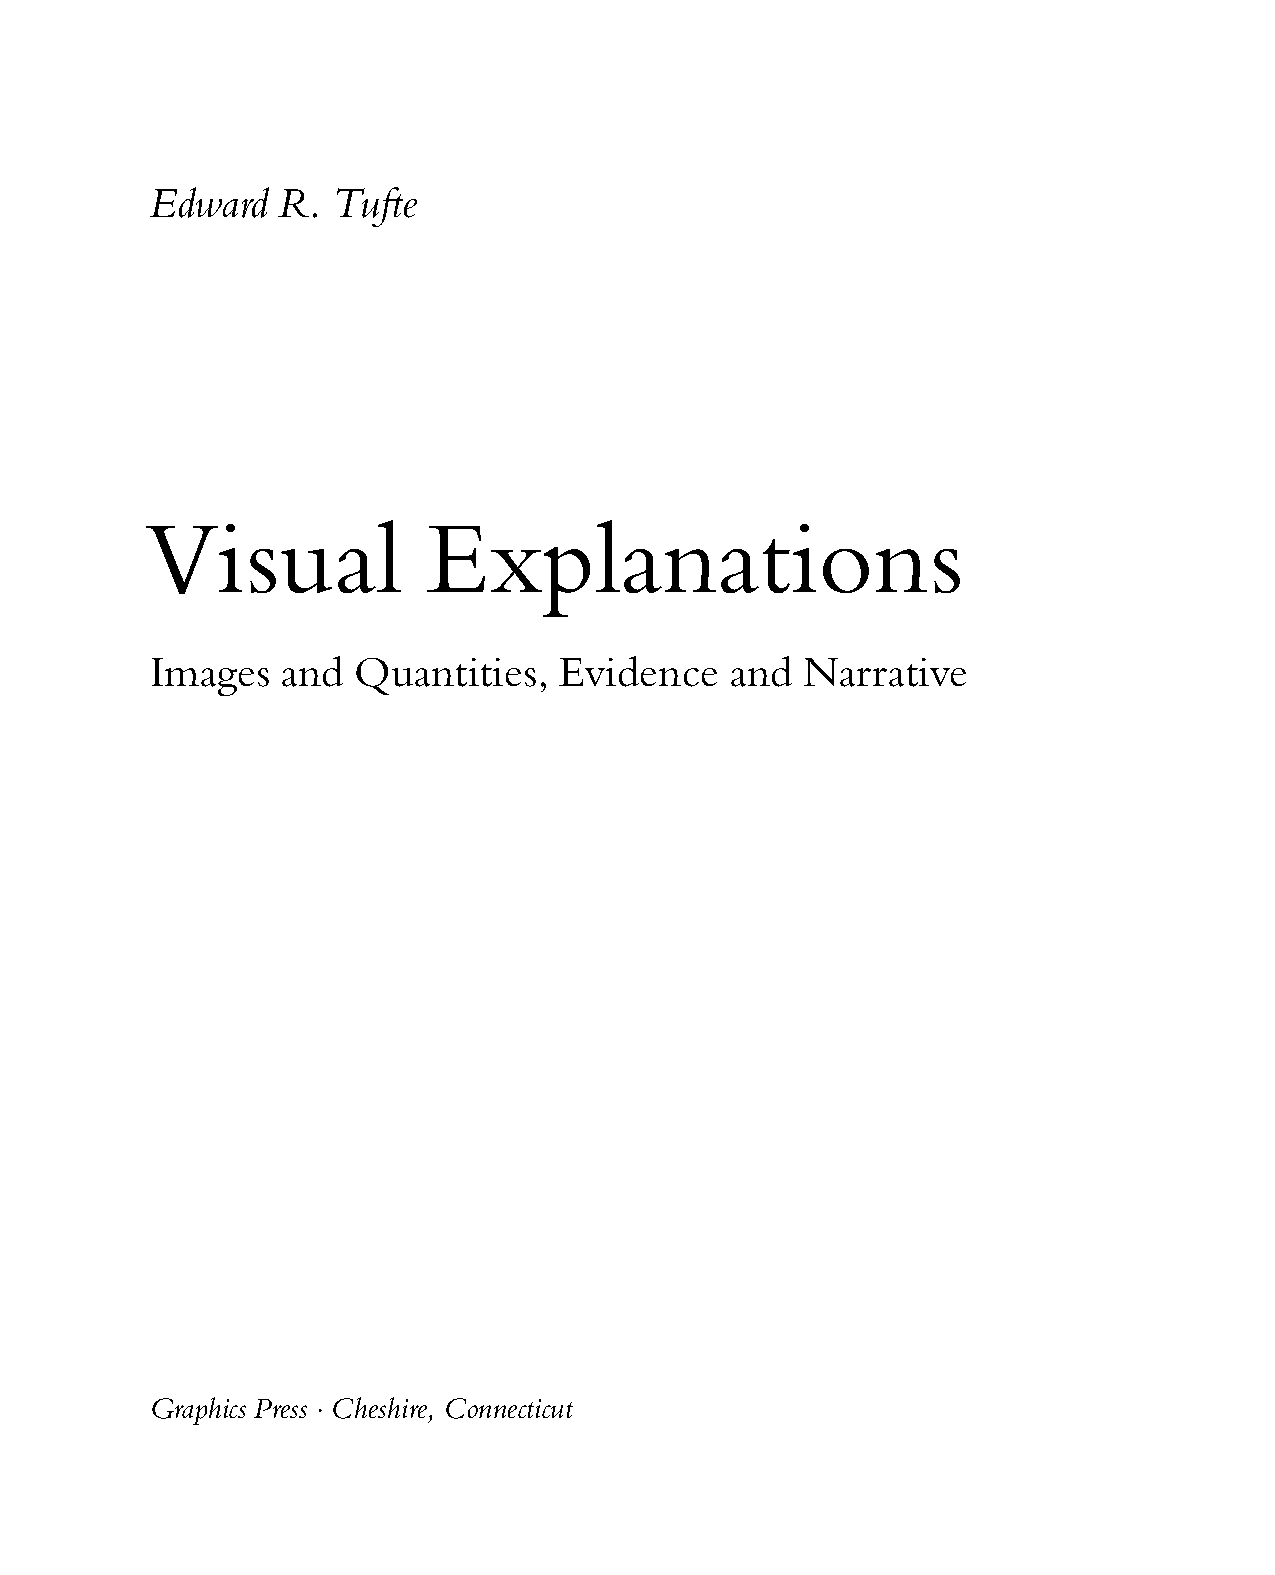
\includegraphics[width=0.45\linewidth,height=\textheight,keepaspectratio]{style-guide/graphics/ve-title.pdf}

\includegraphics[width=0.45\linewidth,height=\textheight,keepaspectratio]{style-guide/graphics/be-title.pdf}

\end{figure*}%

\newthought{The tables of contents} in Tufte's books give us our first
glimpse of the structure of the main matter. \VDQI is split into two
parts, each containing some number of chapters. His other three books
only contain chapters---they're not broken into parts.

\begin{figure*}

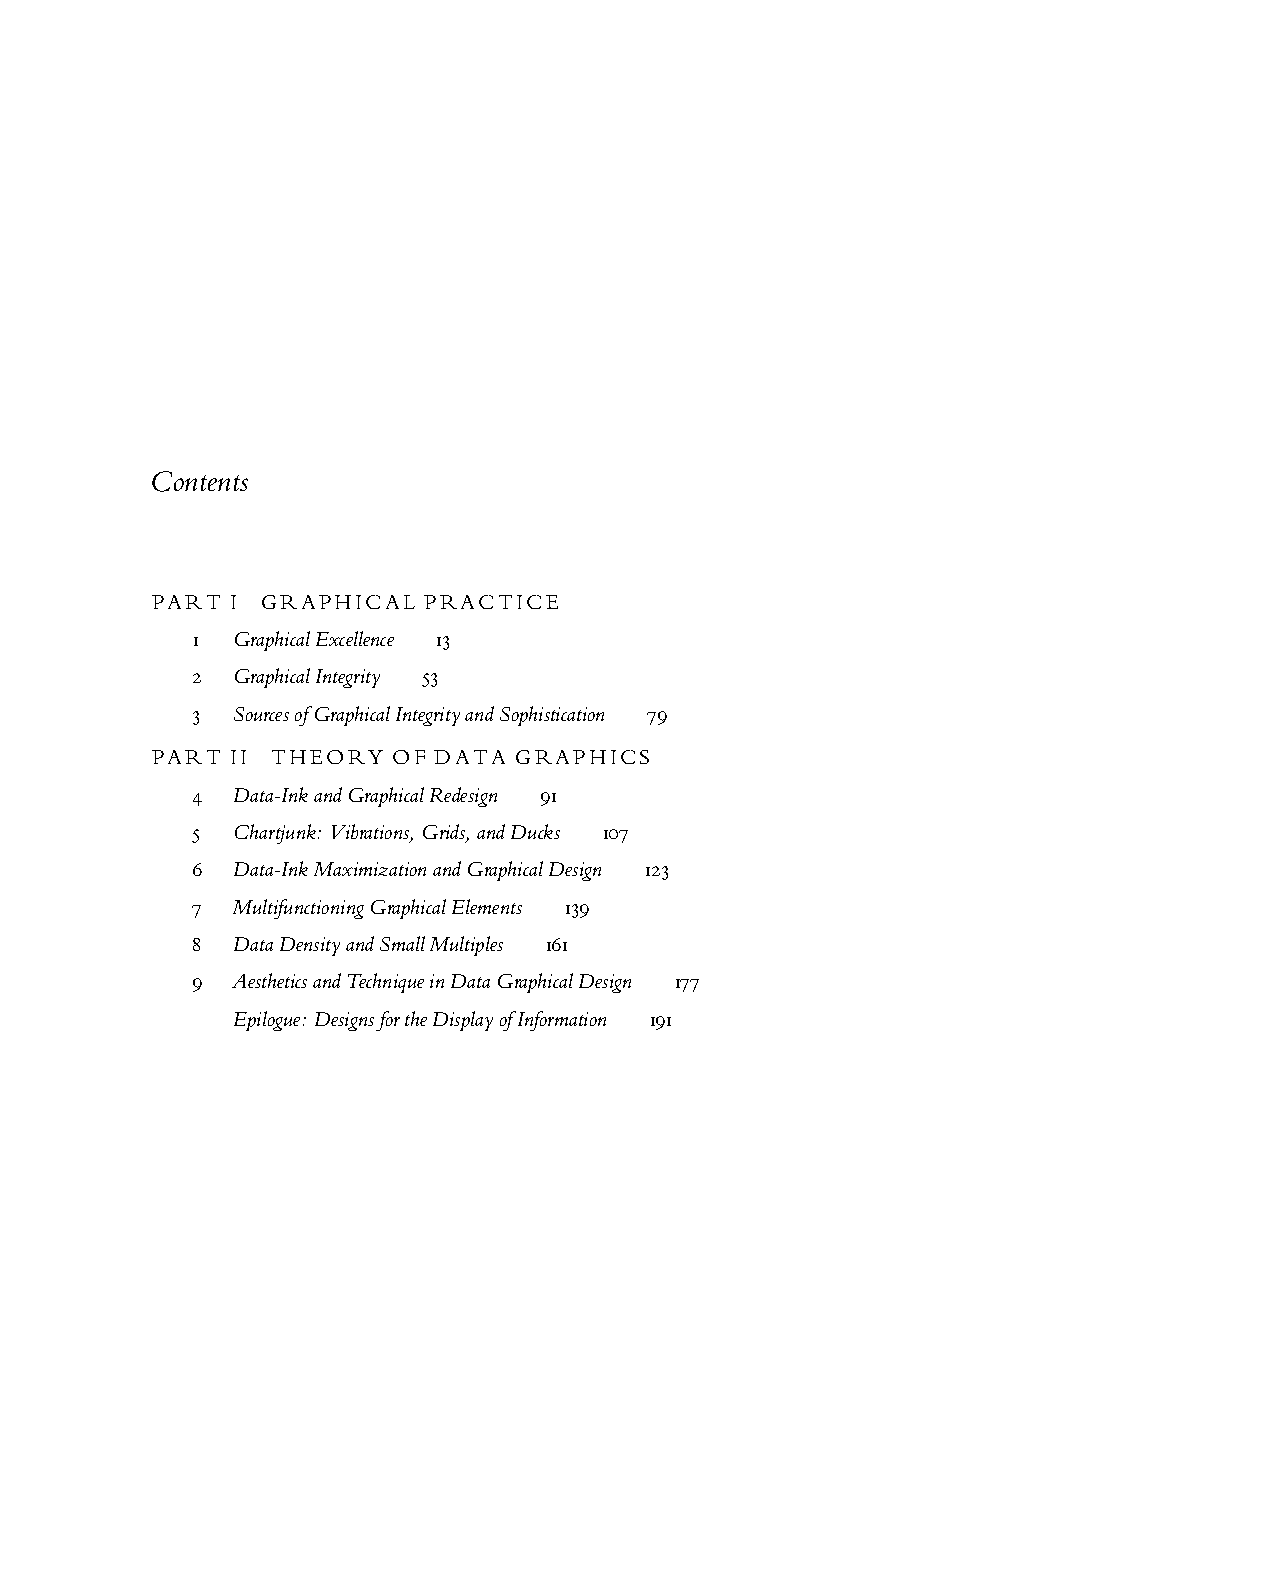
\includegraphics[width=0.45\linewidth,height=\textheight,keepaspectratio]{style-guide/graphics/vdqi-contents.pdf}
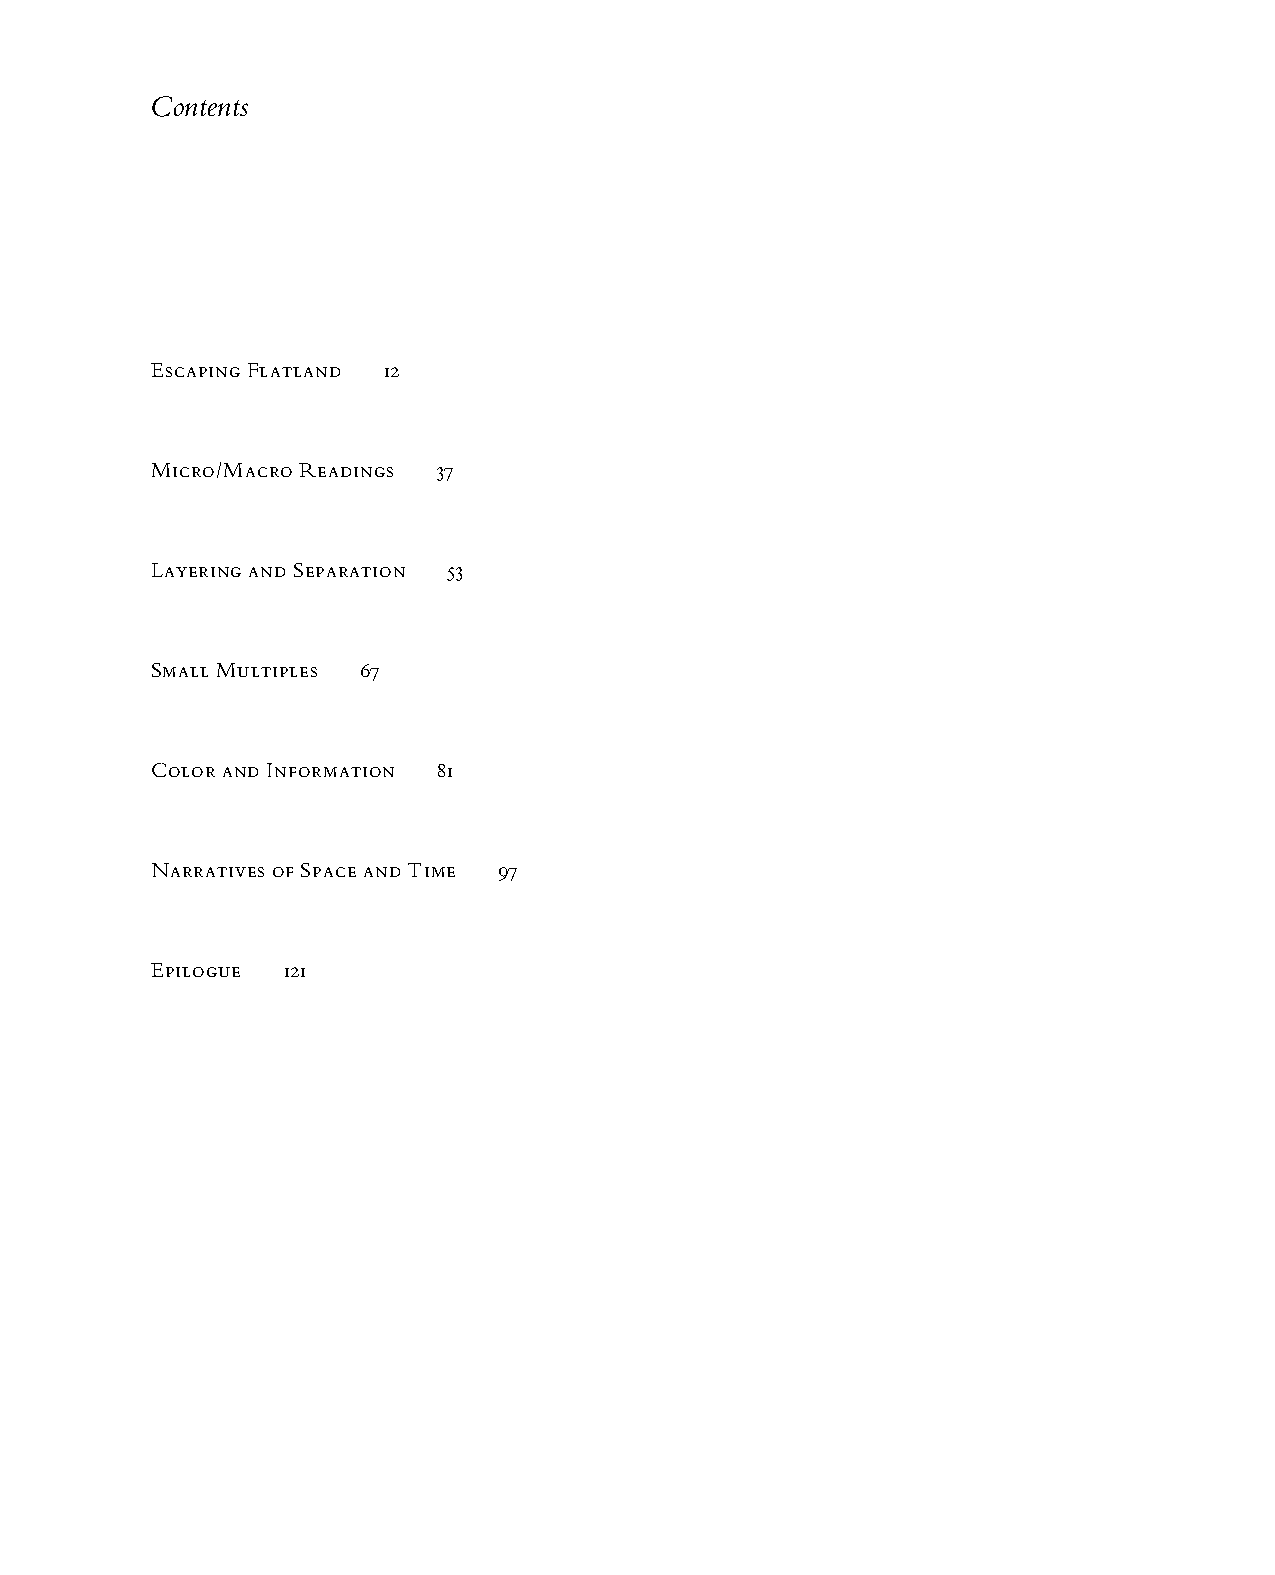
\includegraphics[width=0.45\linewidth,height=\textheight,keepaspectratio]{style-guide/graphics/ei-contents.pdf}

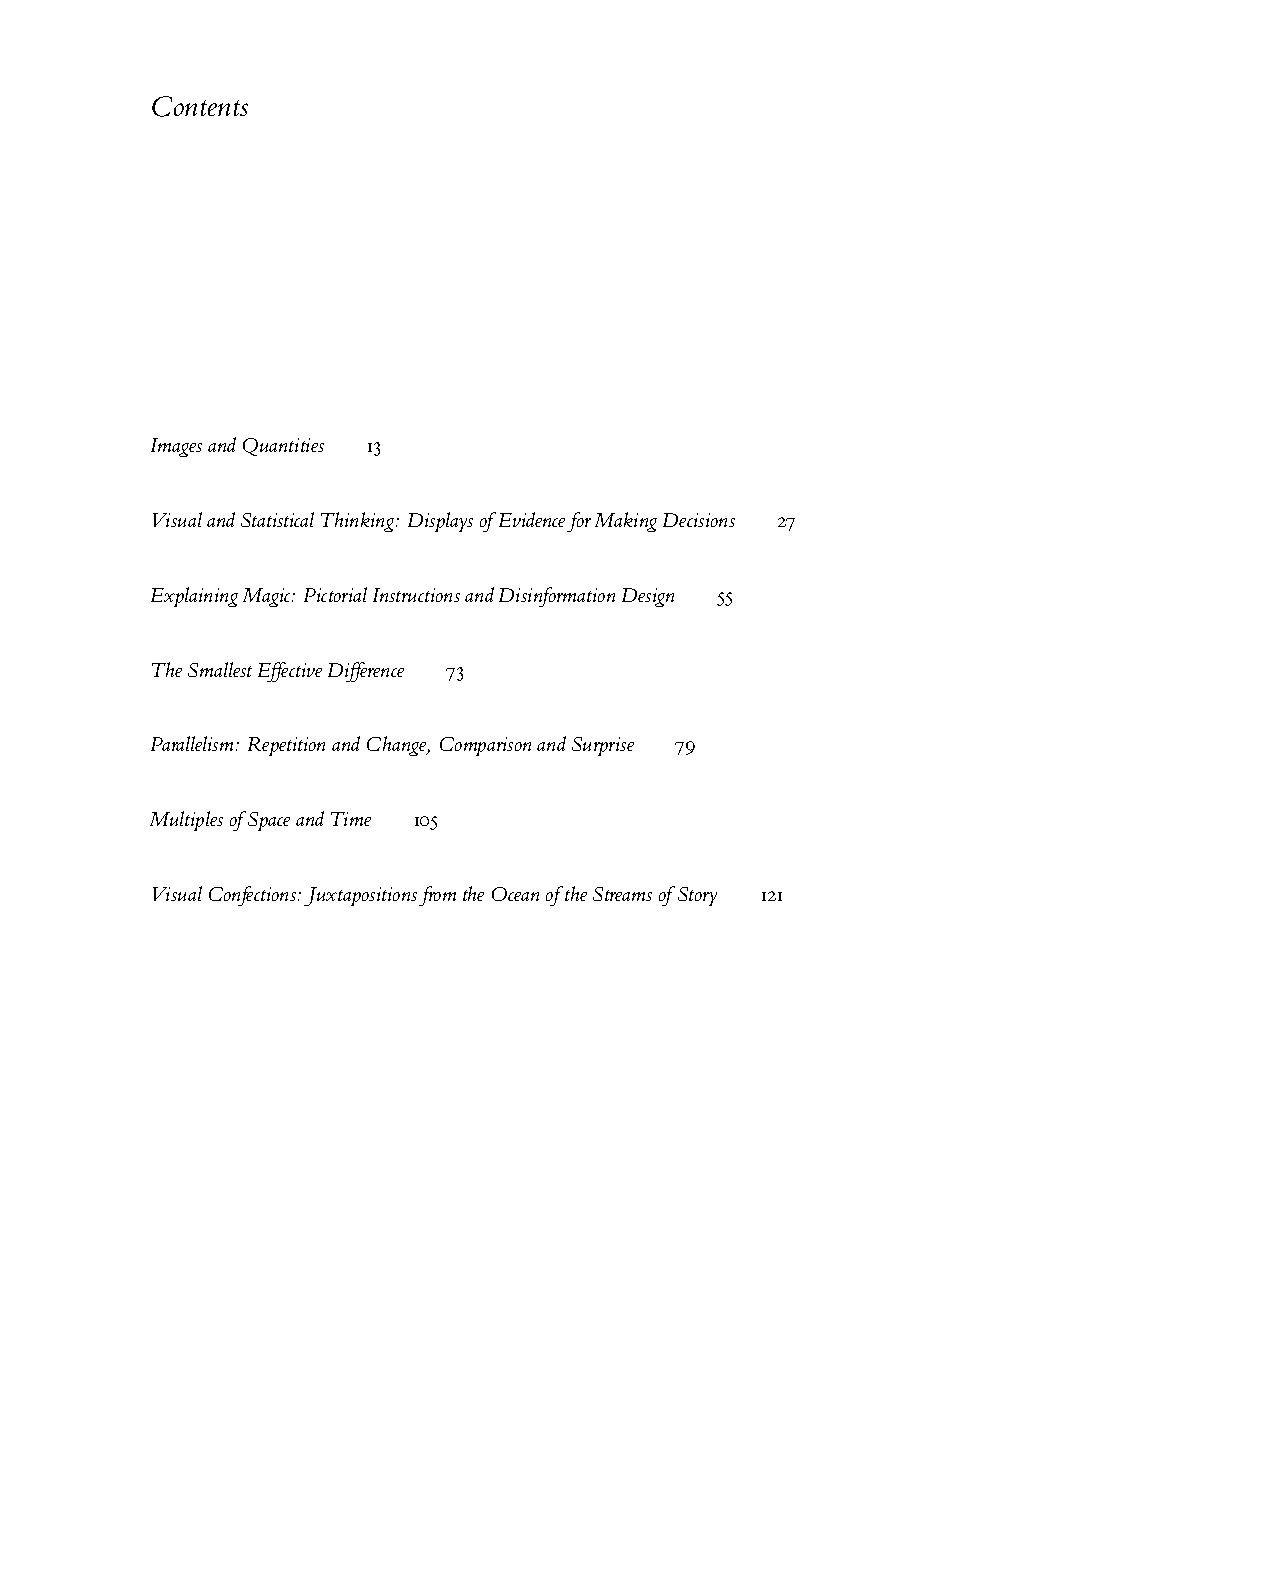
\includegraphics[width=0.45\linewidth,height=\textheight,keepaspectratio]{style-guide/graphics/ve-contents.pdf}
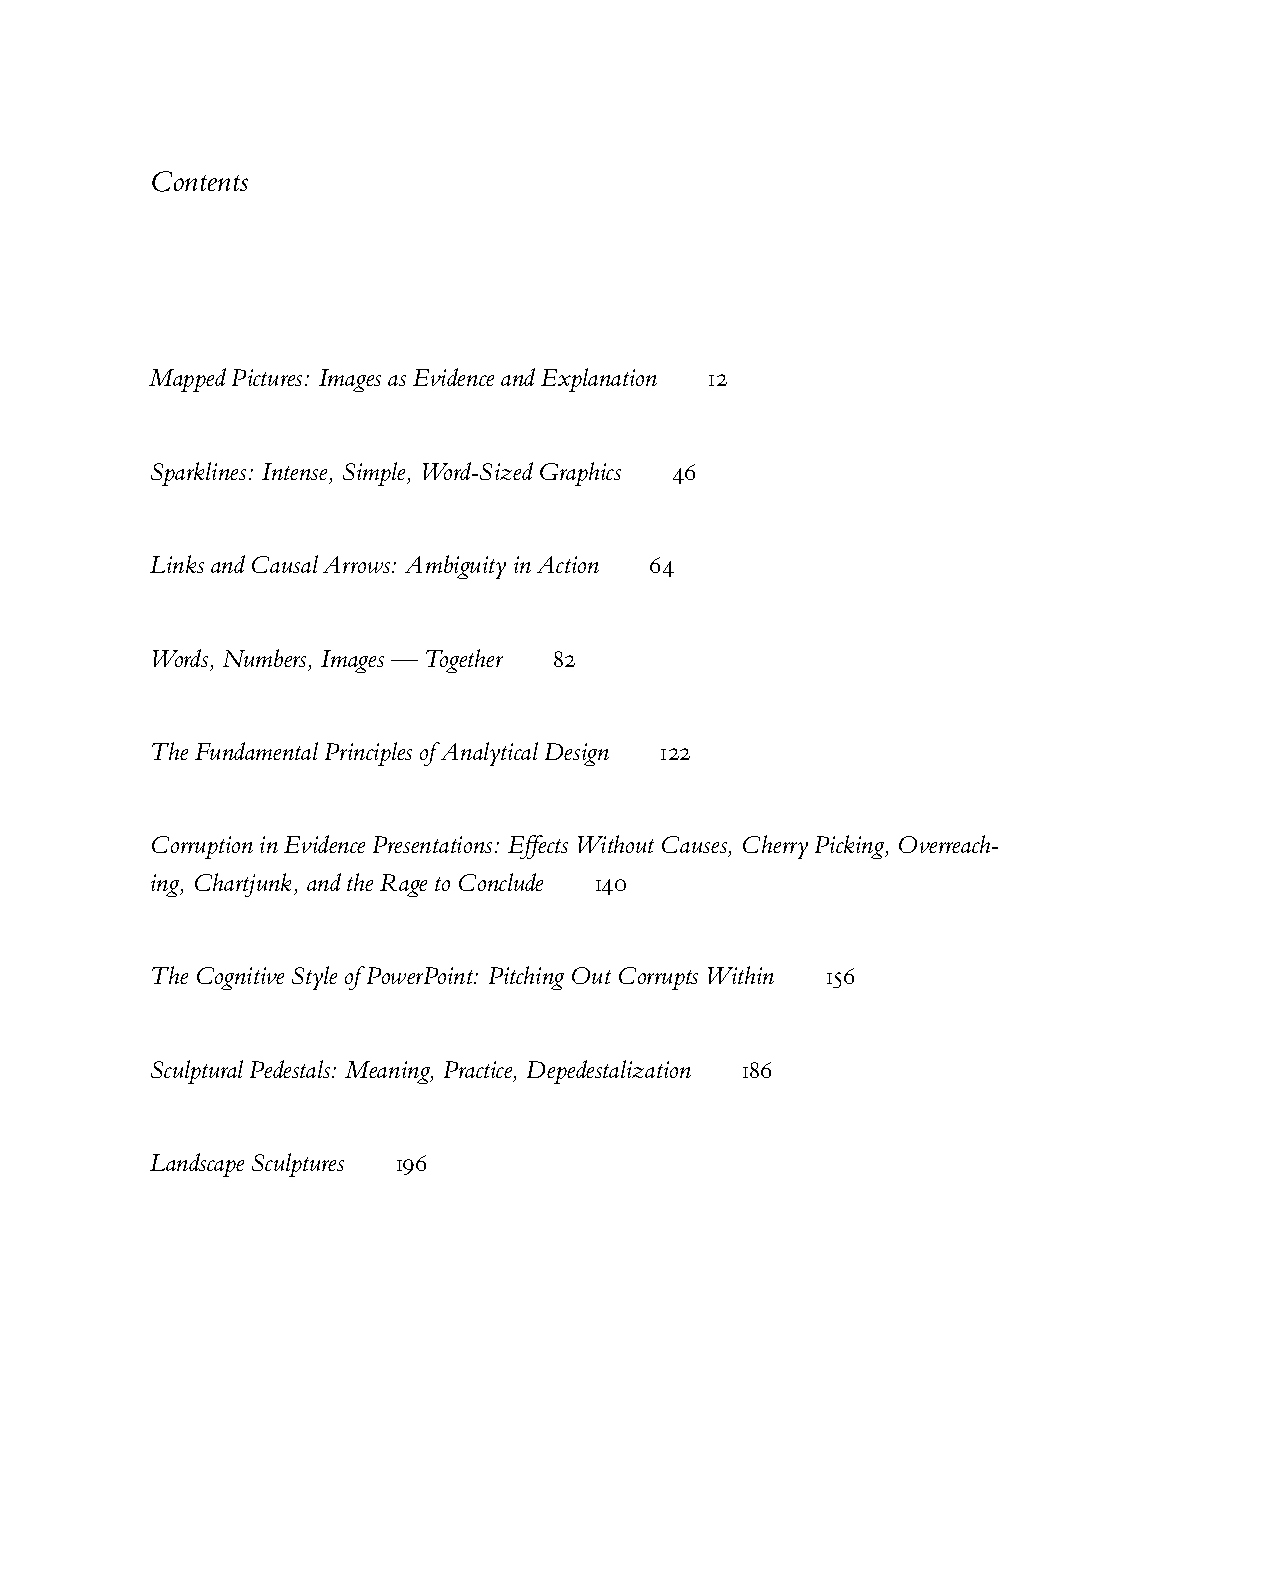
\includegraphics[width=0.45\linewidth,height=\textheight,keepaspectratio]{style-guide/graphics/be-contents.pdf}

\end{figure*}%

\section{Typefaces}\label{sec:typefaces1}

Tufte's books primarily use two typefaces: Bembo and Gill Sans. Bembo is
used for the headings and body text, while Gill Sans is used for the
title page and opening epigraphs in \BE.

Since neither Bembo nor Gill Sans are available in default LaTeX
installations, the \TL document classes default to using Palatino and
Helvetica, respectively. In addition, the Bera Mono typeface is used for
\texttt{monospaced} type.

The following font sizes are defined by the \TL classes:

\begin{table}[h]
\footnotesize
\begin{center}
\begin{tabular}{lccl}
\toprule
\LaTeX{} size & Font size & Leading & Used for \\
\midrule
\verb+\tiny+         &  5 &  6 & sidenote numbers \\
\verb+\scriptsize+   &  7 &  8 & \na \\
\verb+\footnotesize+ &  8 & 10 & sidenotes, captions \\
\verb+\small+        &  9 & 12 & quote, quotation, and verse environments \\
\verb+\normalsize+   & 10 & 14 & body text \\
\verb+\large+        & 11 & 15 & \textsc{b}-heads \\
\verb+\Large+        & 12 & 16 & \textsc{a}-heads, \textsc{toc} entries, author, date \\
\verb+\LARGE+        & 14 & 18 & handout title \\
\verb+\huge+         & 20 & 30 & chapter heads \\
\verb+\Huge+         & 24 & 36 & part titles \\
\bottomrule
\end{tabular}
\end{center}
\caption{A list of \LaTeX{} font sizes as defined by the \TL document classes.}
\label{tab:font-sizes}
\end{table}

\section{Headings}\label{sec:headings1}

Tufte's books include the following heading levels: parts,
chapters\footnote{Parts and chapters are defined for the
  \texttt{tufte-book} class only.}, sections, subsections, and
paragraphs. Not defined by default are: sub-subsections and
subparagraphs.

\begin{table}[h]
\begin{center}
\footnotesize
\begin{tabular}{lcr}
\toprule
Heading & Style & Size \\
\midrule
Part & roman & \measure{24}{36}{40} \\
Chapter & italic & \measure{20}{30}{40} \\
Section & italic & \measure{12}{16}{26} \\
Subsection & italic & \measure{11}{15}{26} \\
Paragraph & italic & 10/14 \\
\bottomrule
\end{tabular}
\end{center}
\caption{Heading styles used in \BE.}
\label{tab:heading-styles}
\end{table}

\subsection*{Paragraph}\label{paragraph}
\addcontentsline{toc}{subsection}{Paragraph}

Paragraph headings (as shown here) are introduced by italicized text and
separated from the main paragraph by a bit of space.

\section{Environments}\label{environments}

The following characteristics define the various environments:

\begin{table}[h]
\begin{center}
\footnotesize
\begin{tabular}{lcl}
\toprule
Environment & Font size & Notes \\
\midrule
Body text & \measure{10}{14}{26} & \\
Block quote & \measure{9}{12}{24} & Block indent (left and right) by \unit[1]{pc} \\
Sidenotes & \measure{8}{10}{12} & Sidenote number is set inline, followed by word space \\
Captions & \measure{8}{10}{12} &  \\
\bottomrule
\end{tabular}
\end{center}
\caption{Environment styles used in \BE.}
\label{tab:environment-styles}
\end{table}

\chapter{On the Use of the tufte-book Document
Class}\label{ch:tufte-book}

The \TL document classes define a style similar to the style Edward
Tufte uses in his books and handouts. Tufte's style is known for its
extensive use of sidenotes, tight integration of graphics with text, and
well-set typography. This document aims to be at once a demonstration of
the features of the \TL document classes and a style guide to their use.

\section{Page Layout}\label{sec:page-layout}

\subsection{Headings}\label{sec:headings}

This style provides \textsc{a}- and \textsc{b}-heads (that is,
\texttt{\textbackslash{}section} and
\texttt{\textbackslash{}subsection}), demonstrated above.

If you need more than two levels of section headings, you'll have to
define them yourself at the moment; there are no pre-defined styles for
anything below a \texttt{\textbackslash{}subsection}. As Bringhurst
points out in \emph{The Elements of Typographic Style}(Bringhurst 2005),
you should ``use as many levels of headings as you need: no more, and no
fewer.''

The \TL classes will emit an error if you try to use
\texttt{\textbackslash{}subsubsection} and smaller headings.

\newthought{In his later books}(Tufte 2006), Tufte starts each section
with a bit of vertical space, a non-indented paragraph, and sets the
first few words of the sentence in \textsc{small caps}. To accomplish
this using this style, use the \texttt{\textbackslash{}newthought}
command.

\section{Sidenotes}\label{sec:sidenotes}

One of the most prominent and distinctive features of this style is the
extensive use of sidenotes. There is a wide margin to provide ample room
for sidenotes and small figures. Any footnotes will automatically be
converted to sidenotes.\footnote{This is a sidenote that was entered
  using the footnote command.} If you'd like to place ancillary
information in the margin without the sidenote mark (the superscript
number), you can use the \texttt{\textbackslash{}marginnote} command.

This is a margin note. Notice that there isn't a number preceding the
note, and there is no number in the main text where this note was
written.

The specification of the \texttt{\textbackslash{}sidenote} command is:

\begin{verbatim}
\sidenote[<number>][<offset>]{<Sidenote text.>}
\end{verbatim}

Both the optional \texttt{number} and \texttt{offset} arguments are
optional. If you provide a \texttt{number} argument, then that number
will be used as the sidenote number. It will change the number of the
current sidenote only and will not affect the numbering sequence of
subsequent sidenotes.

Sometimes a sidenote may run over the top of other text or graphics in
the margin space. If this happens, you can adjust the vertical position
of the sidenote by providing a dimension in the \texttt{offset}
argument. Some examples of valid dimensions are:

\begin{verbatim}
1.0in    2.54cm    254mm    6\baselineskip
\end{verbatim}

If the dimension is positive it will push the sidenote down the page; if
the dimension is negative, it will move the sidenote up the page.

\section{References}\label{references}

References are placed alongside their citations as sidenotes, as
well.\footnote{The first paragraph of this document includes a citation.}
This can be accomplished using the normal \texttt{\textbackslash{}cite}
command.

The complete list of references may also be printed automatically by
using the \texttt{\textbackslash{}bibliography} command. (See the end of
this document for an example.) If you do not want to print a
bibliography at the end of your document, use the
\texttt{\textbackslash{}nobibliography} command in its place.

\section{Figures and Tables}\label{sec:figures-and-tables}

Images and graphics play an integral role in Tufte's work. In addition
to the standard figure and tabular environments, this style provides
special figure and table environments for full-width floats.

Full page-width figures and tables may be placed in \texttt{figure*} or
\texttt{table*} environments. To place figures or tables in the margin,
use the \texttt{marginfigure} or \texttt{margintable} environments as
follows:

\begin{figure}

{\centering \pandocbounded{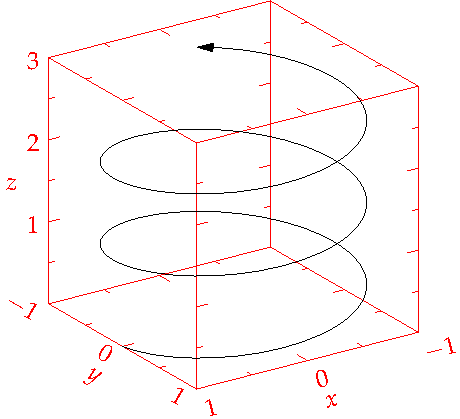
\includegraphics[keepaspectratio]{style-guide/graphics/helix.pdf}}

}

\caption{This is a margin figure. The helix is defined by
\(x = \cos(2\pi z)\), \(y = \sin(2\pi z)\), and \(z = [0, 2.7]\). The
figure was drawn using Asymptote (http://asymptote.sf.net/).}

\end{figure}%

The \texttt{marginfigure} and \texttt{margintable} environments accept
an optional parameter that adjusts the vertical position of the figure
or table. See the ``Sidenotes'' section above for examples.

Figure (\textbf{fig:fullfig?}) is an example of a full-width figure and
Figure (\textbf{fig:textfig?}) is an example of the normal figure
environment.

\begin{figure*}

\begin{figure}

{\centering \pandocbounded{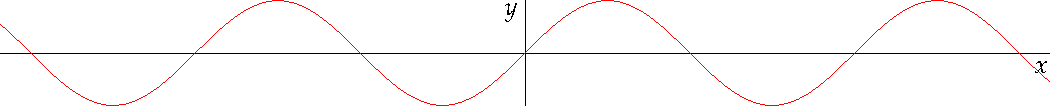
\includegraphics[keepaspectratio]{style-guide/graphics/sine.pdf}}

}

\caption{This graph shows \(y = \sin x\) from about \(x = [-10, 10]\).
\emph{Notice that this figure takes up the full page width.}}

\end{figure}%

\end{figure*}%

\begin{figure}

{\centering \pandocbounded{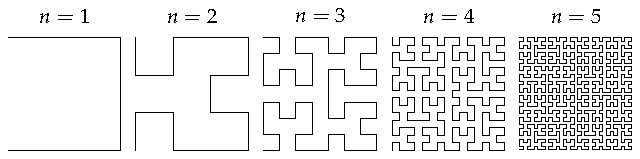
\includegraphics[keepaspectratio]{style-guide/graphics/hilbertcurves.pdf}}

}

\caption{Hilbert curves of various degrees \(n\). \emph{Notice that this
figure only takes up the main textblock width.}}

\end{figure}%

Table (\textbf{tbl:normaltab?}) shows a table created with the
\texttt{booktabs} package. Notice the lack of vertical rules---they
serve only to clutter the table's data.

\begin{table}[ht]
\centering
\fontfamily{ppl}\selectfont
\begin{tabular}{ll}
\toprule
Margin & Length \\
\midrule
Paper width & \unit[8\nicefrac{1}{2}]{inches} \\
Paper height & \unit[11]{inches} \\
Textblock width & \unit[6\nicefrac{1}{2}]{inches} \\
Textblock/sidenote gutter & \unit[\nicefrac{3}{8}]{inches} \\
Sidenote width & \unit[2]{inches} \\
\bottomrule
\end{tabular}
\caption{Here are the dimensions of the various margins used in the Tufte-handout class.}
\label{tab:normaltab}
\end{table}

\newthought{Occasionally} LaTeX will generate an error message:

\begin{verbatim}
Error: Too many unprocessed floats
\end{verbatim}

LaTeX tries to place floats in the best position on the page. Until it's
finished composing the page, however, it won't know where those
positions are. If you have a lot of floats on a page (including
sidenotes, margin notes, figures, tables, etc.), LaTeX may run out of
``slots'' to keep track of them and will generate the above error.

\section{Typography}\label{sec:typography}

\subsection{Typefaces}\label{sec:typefaces}

If the Palatino, Helvetica, and Bera Mono typefaces are installed, this
style will use them automatically. Otherwise, we'll fall back on the
Computer Modern typefaces.

\subsection{Letterspacing}\label{sec:letterspacing}

This document class includes two new commands and some improvements on
existing commands for letterspacing.

When setting strings of \allcaps{ALL CAPS} or \smallcaps{small caps},
the letterspacing---that is, the spacing between the letters---should be
increased slightly(Bringhurst 2005). The
\texttt{\textbackslash{}allcaps} command has proper letterspacing for
strings of \allcaps{FULL CAPITAL LETTERS}, and the
\texttt{\textbackslash{}smallcaps} command has letterspacing for
\smallcaps{small capital letters}. These commands will also
automatically convert the case of the text to upper- or lowercase,
respectively.

\section{Document Class Options}\label{sec:options}

The \texttt{tufte-book} class is based on the LaTeX \texttt{book}
document class. Therefore, you can pass any of the typical book options.
There are a few options that are specific to the \texttt{tufte-book}
document class, however.

The \texttt{a4paper} option will set the paper size to \smallcaps{A4}
instead of the default \smallcaps{US} letter size.

The \texttt{sfsidenotes} option will set the sidenotes and title block
in a sans serif typeface instead of the default roman.

The \texttt{twoside} option will modify the running heads so that the
page number is printed on the outside edge (as opposed to always
printing the page number on the right-side edge in \texttt{oneside}
mode).

The \texttt{symmetric} option typesets the sidenotes on the outside edge
of the page. This is how books are traditionally printed, but is
contrary to Tufte's book design which sets the sidenotes on the right
side of the page. This option implicitly sets the \texttt{twoside}
option.

The \texttt{justified} option sets all the text fully justified (flush
left and right). The default is to set the text ragged right. The body
text of Tufte's books are set ragged right. This prevents needless
hyphenation and makes it easier to read the text in the slightly
narrower column.

\chapter*{References}\label{references-1}
\addcontentsline{toc}{chapter}{References}

\phantomsection\label{refs}
\begin{CSLReferences}{1}{0}
\bibitem[\citeproctext]{ref-Bringhurst2005}
Bringhurst, Robert. 2005. \emph{The Elements of Typography}. 3.1 ed.
Hartley \& Marks.

\bibitem[\citeproctext]{ref-Tufte1990}
Tufte, Edward R. 1990. \emph{Envisioning Information}. Cheshire,
Connecticut: Graphics Press.

\bibitem[\citeproctext]{ref-Tufte1997}
---------. 1997. \emph{Visual Explanations}. Cheshire, Connecticut:
Graphics Press.

\bibitem[\citeproctext]{ref-Tufte2001}
---------. 2001. \emph{The Visual Display of Quantitative Information}.
Cheshire, Connecticut: Graphics Press.

\bibitem[\citeproctext]{ref-Tufte2006}
---------. 2006. \emph{Beautiful Evidence}. First. Graphics Press,
{LLC}.

\end{CSLReferences}


\backmatter


\end{document}
